\documentclass[a4paper]{jpconf}
\usepackage{graphicx}
\usepackage{fancyvrb}
\usepackage{xcolor}

\xdefinecolor{dianablue}{rgb}{0.18,0.24,0.31}
\xdefinecolor{darkblue}{rgb}{0.1,0.1,0.7}
\xdefinecolor{darkgreen}{rgb}{0,0.5,0}
\xdefinecolor{darkgrey}{rgb}{0.35,0.35,0.35}
\xdefinecolor{darkorange}{rgb}{0.8,0.5,0}
\xdefinecolor{darkorange2}{rgb}{1,0.5,0}
\xdefinecolor{darkred}{rgb}{0.7,0,0}
\xdefinecolor{darkpink}{rgb}{0.9,0.2,0.6}
\definecolor{darkgreen}{rgb}{0,0.6,0}
\definecolor{mauve}{rgb}{0.58,0,0.82}

\begin{document}
\title{Nested data structures in array frameworks}

\author{Jim Pivarski, David Lange, and Peter Elmer}

\address{Princeton University}

\ead{pivarski@princeton.edu, david.lange@cern.ch, peter.elmer@cern.ch}

\begin{abstract}
The need for nested data structures and combinatorial operations on arbitrary length lists has prevented particle physicists from widely adopting data analysis languages, such as R, MATLAB, Numpy, and Pandas. These array frameworks work well for purely rectangular tables and hypercubes, but arrays of variable length arrays, called ``jagged arrays,'' are out of their scope. However, jagged arrays are a fundamental feature of particle physics data, as well as combining them to search for particle decays. To bridge this gap, we have developed the awkward-array library, and in this paper we present feedback from the first physics groups using it for their analyses. They report similar computational performance between analysis code written in C++ and array-based analysis scripts written entirely in Python, and are split on the ease-of-use of array syntax. In a series of four phone interviews, all users noted how different array programming is from imperative programming, but whereas some found it much easier, others said it was more difficult to write, yet easier to read.
\end{abstract}

\section{Structure of data in particle physics}

Data analysis software intended for data scientists and big data analyses is mostly designed for simple data that must be cross-correlated in complex ways. By contrast, particle physicists deal with strictly independent events that are nevertheless complex within those events. This allows them more freedom in parallel processing, but they requrie more specialized tools to run in those parallel jobs. Particle physicists usually solve this problem by writing imperative code in a general purpose programming language, typically C++, as the first step in their data analyses.

There is much to be gained from higher level analysis tools, but physicists cannot use them if they do not represent and provide operations for complex data. ``Complex data'' involves several features:
\begin{itemize}
\item collections of variable length arrays, to represent arbitrary numbers of particles per event and similar structures;
\item nested record types for particle objects;
\item cross-linked data, such as pointers from jet objects to the tracks that comprise them;
\item nullable data, such as a parameter value from a fit that did not converge.
\end{itemize}

All of these are easy to deal with as simple numerical types except the first, known as ``jagged arrays.'' Nested record types, such as a {\tt lorentz} field containing objects with {\tt pt}, {\tt phi}, and {\tt eta} fields, could be thought of as a naming convention, as field names containing dots: {\tt lorentz.pt}, {\tt lorentz.phi}, and {\tt lorentz.eta}. Cross-linked data can be---and frequently are---represented as integers indicating positions in another collection (i.e.\ relational normalization with array index position as the surrogate key). Null values in data are usually indicated by a dummy value, such as $-1000$. Therefore, jagged arrays need the most attention.

\section{Jagged arrays and the awkward-array library}

Jagged arrays can be represented in flat arrays without padding or truncation by separating the content from the structure. Figure~\ref{fig:muons} shows the deconstruction of several muon objects per event as an example. Each nested record has three fields, which can be placed in separate arrays because nested records are essentially a naming convention. The structural part, the fact that the first event has 3 muons, the second has 1, the third has 1, and the fourth has 2, could be recorded in a separate {\tt counts} array. The cumulative sum of {\tt counts}, called {\tt offsets} in the Figure, is more useful because it permits random access: to get the third event (index {\tt 2}), we query {\tt offsets[2]}, which is {\tt 4}. The content for this event starts in $p_T$, phi, and eta arrays at index {\tt 4}.

\begin{figure}
\begin{center}

\begin{minipage}{0.97\linewidth}
\small
\begin{Verbatim}[commandchars=\\\{\},frame=single]
muons = [
 [Muon(\textcolor{darkgreen}{31.1}, \textcolor{darkorange}{-0.481}, \textcolor{blue}{0.882}), Muon(\textcolor{darkgreen}{9.76}, \textcolor{darkorange}{-0.124}, \textcolor{blue}{0.924}), Muon(\textcolor{darkgreen}{8.18}, \textcolor{darkorange}{-0.119}, \textcolor{blue}{0.923})],
 [Muon(\textcolor{darkgreen}{5.27}, \textcolor{darkorange}{1.246}, \textcolor{blue}{-0.991})],
 [Muon(\textcolor{darkgreen}{4.72}, \textcolor{darkorange}{-0.207}, \textcolor{blue}{0.953})],
 [Muon(\textcolor{darkgreen}{8.59}, \textcolor{darkorange}{-1.754}, \textcolor{blue}{-0.264}), Muon(\textcolor{darkgreen}{8.714}, \textcolor{darkorange}{0.185}, \textcolor{blue}{0.629})],
 ...
]
\end{Verbatim}
\end{minipage}

\vspace{0.5 cm}
\renewcommand{\arraystretch}{1.25}
\begin{tabular}{| r | l |}
\hline
\mbox{\hspace{1 cm}$p_T$} & \textcolor{darkgreen}{\tt \ \ 31.1,\ \ \ 9.76,\ \ \ 8.18,\ \ \ 5.27,\ \ \ 4.72,\ \ \ 8.59, 8.714} \\
phi &  \textcolor{darkorange}{\tt -0.481,\ -0.123,\ -0.119,\ \ 1.246,\ -0.207,\ -1.754,\ 0.185} \\
eta &        \textcolor{blue}{\tt \ 0.882,\ \ 0.924,\ \ 0.923,\ -0.991,\ \ 0.953,\ -0.264,\ 0.629} \\\hline
{\tt counts}  & \tt \ \ \ \ \ 3,\ \ \ \ \ \ \ \ \ \ \ \ \ \ \ \ \ \ \ \ \ \ 1,\ \ \ \ \ \ 1,\ \ \ \ \ \ 2\ \ \ \ \ \ \ \ \ \\\hline
{\tt offsets} & \tt \ \ \ \ \ 0,\ \ \ \ \ \ \ \ \ \ \ \ \ \ \ \ \ \ \ \ \ \ 3,\ \ \ \ \ \ 4,\ \ \ \ \ \ 5,\ \ \ \ \ \ \ 7 \\\hline
{\tt starts}  & \tt \ \ \ \ \ 0,\ \ \ \ \ \ \ \ \ \ \ \ \ \ \ \ \ \ \ \ \ \ 3,\ \ \ \ \ \ 4,\ \ \ \ \ \ 5\ \ \ \ \ \ \ \ \ \\
{\tt stops}   & \tt \ \ \ \ \ 3,\ \ \ \ \ \ \ \ \ \ \ \ \ \ \ \ \ \ \ \ \ \ 4,\ \ \ \ \ \ 5,\ \ \ \ \ \ 7\ \ \ \ \ \ \ \ \ \\\hline
{\tt parents} & \tt \ \ \ \ \ 0,\ \ \ \ \ \ 0,\ \ \ \ \ \ 0,\ \ \ \ \ \ 1,\ \ \ \ \ \ 2,\ \ \ \ \ \ 3,\ \ \ \ \ 3 \\\hline
\end{tabular}

\end{center}

\caption{Example of arbitrarily many muon records per event (top code snippet) and their representation as content arrays ($p_T$, phi, eta, bottom table) and structure arrays ({\tt counts}, {\tt offsets}, {\tt starts} and {\tt stops}, or {\tt parents}, bottom table). \label{fig:muons}}
\end{figure}

Some operations that would require expensive rewrites of serialized data structures, such as {\tt std::vector<std::vector<Muon>>}, are simpler and more efficient in array form. For instance, if the {\tt offsets} are separated into {\tt starts} and {\tt stops} (which overlap for all but the first and last entry), dropping all but the leading and subleading particle in each event is a matter of reassigning {\tt stops = min(stops, starts + 2)}. Operations that reduce the structure of the jagged array, such as selecting the best particle per event, require pointers from the inside out, rather than outside in: the {\tt parents} array associates each content value with the event to which it belongs.

Any of these structure arrays can represent the jagged dataset, so a library named awkward-array~\cite{awkward} was developed to manage {\tt JaggedArrays} as a class with similar properties to Numpy's {\tt ndarray}. The awkward-array library handles all of the data structures physicists regularly use---nested records, cross-linked tables, nullable data---but jagged arrays are its primary application. The design of this library is more fully described in our previous paper\cite{2019EPJWC}.

The awkward-array library is used in production, both in the individual cases that will be described later in this paper and also by a large community of physicists. Figure~\ref{fig:uproot} shows pip-installations on computers whose operating system has ``Scientific'' in its name---variants on CERN and Fermi Scientific Linux. Most of these are batch and login machines for particle physicists, so the download rate is driven by distributed analyses. This rate sometimes spikes due to very large jobs, so we smooth it with a 30-day window. In the smoothed time series, we see a steady increase in uproot~\cite{uproot} usage that might be driving a slight increase in Numpy, Matplotlib, and Pandas on these systems. The download rate of awkward-array closely tracks that of uproot, starting when it became a dependency of uproot in version 3.

\begin{figure}
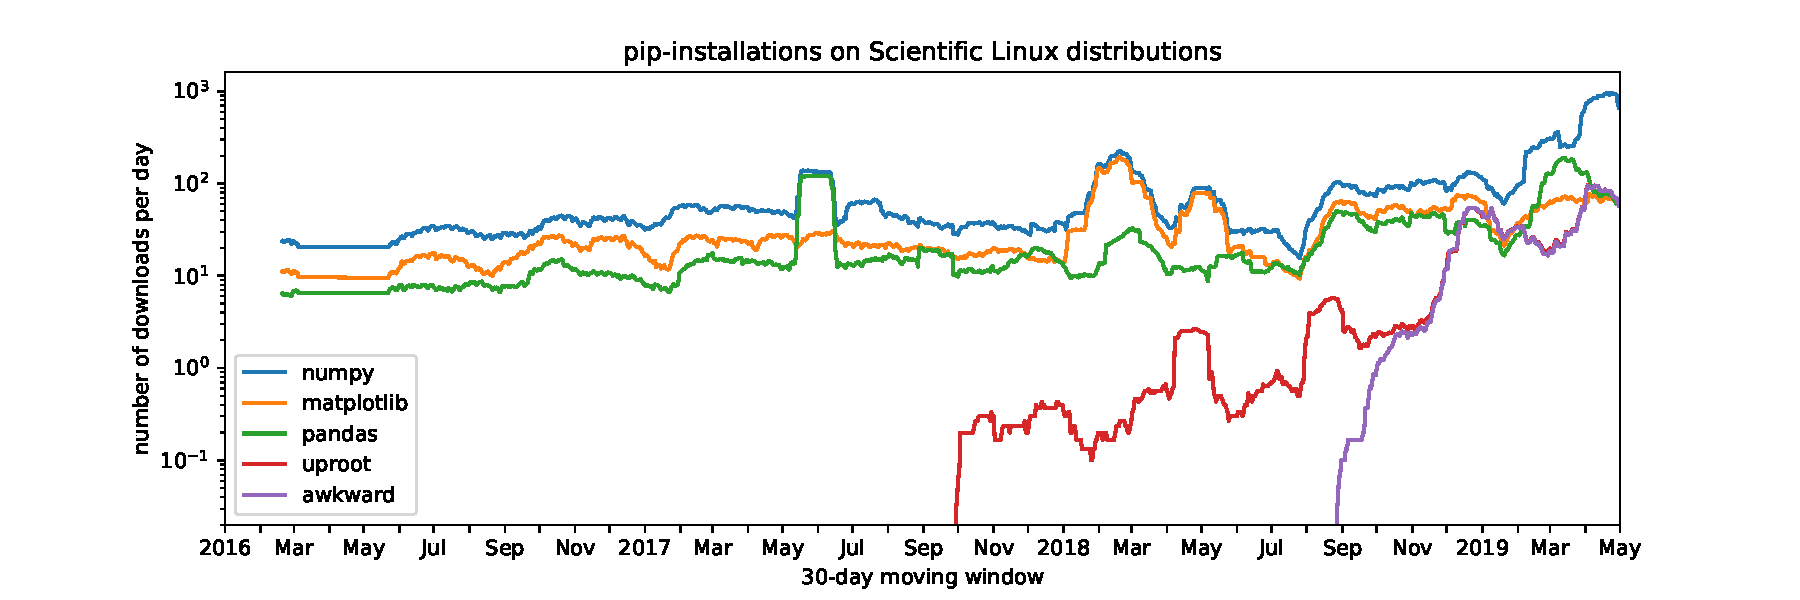
\includegraphics[width=\linewidth]{pip-scientificlinux-uproot.pdf}

\caption{Download rate (30-day window-averaged pip installations per day) of scientific Python libraries on operating systems with ``Scientific'' in their names, including awkward-array. \label{fig:uproot}}
\end{figure}

As we can see from the close tracking of uproot and awkward-array, nearly all awkward-array installations are through the uproot dependency. Some users might not be aware that they are separate libraries: uproot requests return awkward-array objects, primarily {\tt JaggedArrays} and jagged {\tt TLorentzVectorArrays} (which is actually defined in a third dependency: uproot-methods). We cannot tell how many of these users are performing jagged array operations in their analyses, but we can track the usage patterns of a few physicists in depth.

\section{Coffea: awkward-array in two CMS analyses}

Coffea~\cite{coffea} is a collaboration of Fermilab physicists performing two CMS analyses: a dark Higgs search and a boosted Standard Model Higgs $\to$ $b\bar{b}$. The dark Higgs search is being performed exclusively in awkward-array operations, without call-outs to custom C++ code or Python for-loops over the set of events, and the boosted Higgs is being analyzed in parallel with awkward-array and conventional tools, for comparison. This group is also building specialized tools on top of awkward-array for energy corrections, histogramming, and distributed scale-out.









%% \begin{figure}
%% \begin{center}
%% 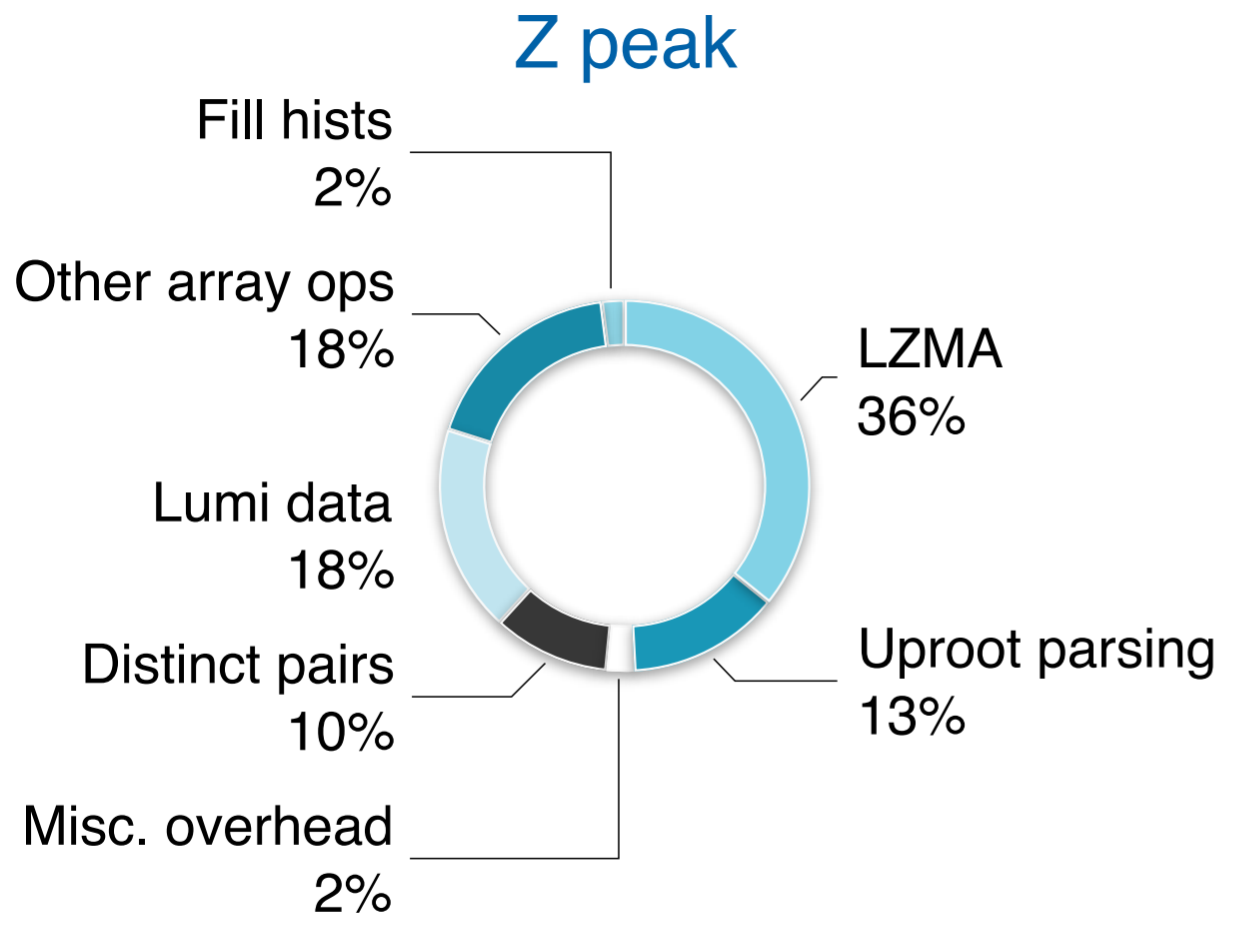
\includegraphics[width=0.5\linewidth]{zpeak-performance-breakdown.png}
%% \end{center}

%% \caption{HERE. \label{fig:zpeak}}
%% \end{figure}




\section{Acknowledgments}

This work was supported by the National Science Foundation under grants ACI-1450377 and PHY-1624356.

\section*{References}
\bibliography{thebibliography}{}
\bibliographystyle{plain}

\end{document}
